\documentclass[a4paper]{report}
\usepackage{listings}
\usepackage{enumitem}
\usepackage{mdframed}
\usepackage{graphicx} % Required for the inclusion of images

\title{CEEN 8886: Homework 5}
\date{2017-04-03}
\author{Kelly Boswell}

\begin{document}

\maketitle

\pagenumbering{gobble}

\newpage

\pagenumbering{arabic}

% Problem 1
\section{Problem 1 --- GSM Security}

Answer the following questions about GSM Security. Refer to \ref{table:prob1} for expansions of any
    acronyms used throughout Problem 1.

\subsection{How is authentication achieved in GSM?}

\begin{table}
\caption{GSM Acronyms and Expansion}
\label{table:prob1}
\begin{center}
\begin{tabular}{| c | l |}
\hline
Acronym & Expansion \\
\hline
IMEI & International Mobile Equipment Identity \\
\hline
$SIM$ & Subscriber Identity Module \\
\hline
$IMSI$ & International Mobile Subscriber Identity \\
\hline
$TMSI$ & Temporary Mobile Subscriber Identity \\
\hline
$PIN$ & Personal Identity Number \\
\hline
$MSC$ & Mobile Switching Center \\
\hline
$HLR$ & Home Location Register \\
\hline
$VLR$ & Visitor Location Register \\
\hline
$AuC$ & Authentication Center \\
\hline
$EIR$ & Equipment Identity Register \\
\hline
$SRES$ & Signed Response \\
\hline
$RAND$ & Random Number \\
\hline
$K_i$ & User's Secret Key \\
\hline
$K_c$ & Ciphering Key \\
\hline
$LAI$ & Location Area Identity \\
\hline
\end{tabular}
\end{center}
\end{table}

GSM authentication follows the following procedure.  See Figure \ref{fig:prob1a} for a high-level depiction of
the protocol. 

\begin{itemize}
\item The $MS$ sends its $IMSI$ to the network subsystem ($AuC$ and $HLR$).
\item The network subsystem receives the $IMSI$ and finds the corresponding $K_i$ of the $IMSI$.
\item The $AuC$ generates a 128-bit $RAND$ and sends the $RAND$, $SRES$, $K_c$ triplet to the $MS$.
\item The $AuC$ calculates the $SRES$ with the $A3$ algorithm.
\item The $MS$ calculates a $SRES$ with $A3$ using $K_i$ and the given $RAND$.
\item The $MS$ sends the $SRES'$ to the network.
\item The visited network compares the $SRES$ and $SRES'$ for verification.
\end{itemize}

\begin{figure}
\begin{mdframed}
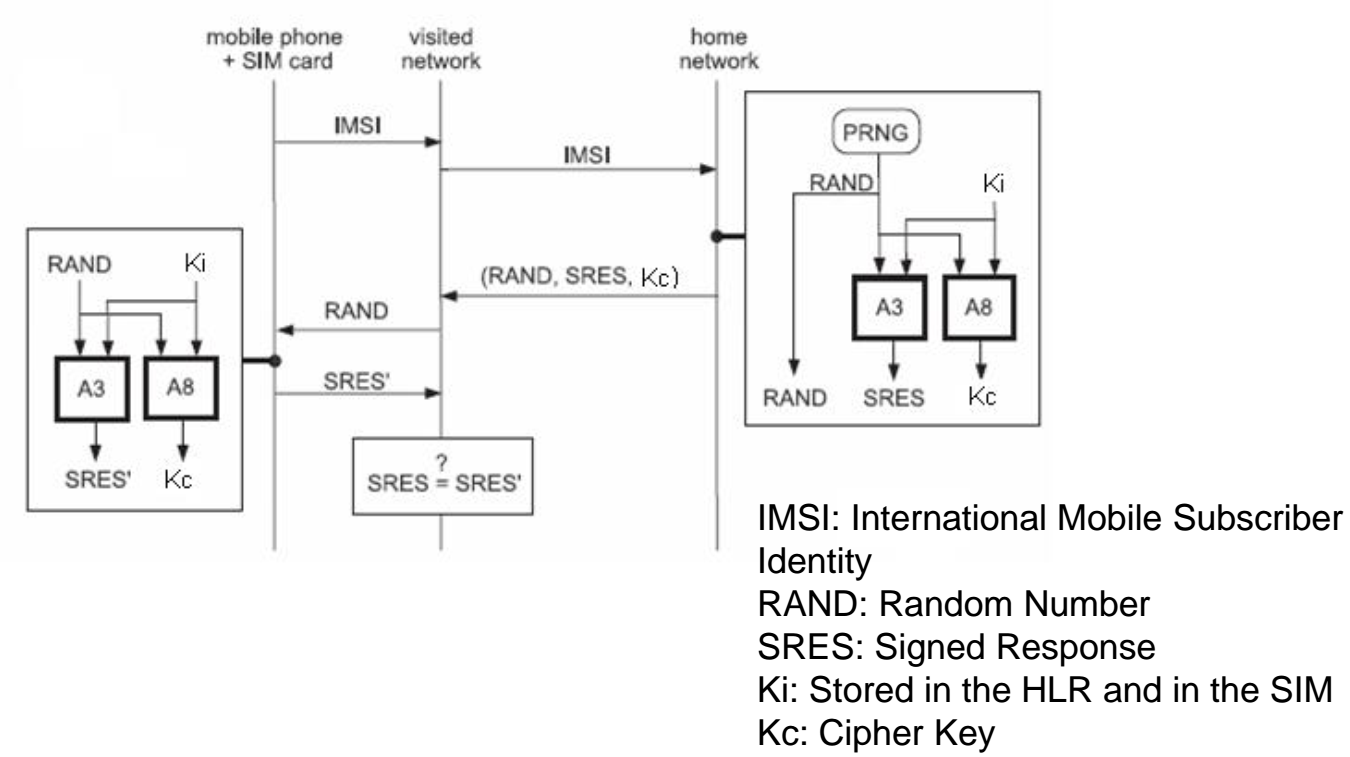
\includegraphics[scale=0.2]{GSM_Authentication_Protocol.png}
\caption{Identifying the SSID information of the WAP.}
\label{fig:prob1a}
\end{mdframed}
\end{figure}

\subsection{Why are the phone calls encrypted?}

To provide confidentiality to the end users.

\subsection{Why is the $SRES$, $RAND$, $K_C$ triplet discarded after being used only once?}

To prevent replay attacks.

\subsection{What is the function of the SIM card in the GSM phone?}

It contains all data specific to the end user which have to reside in the Mobile Station:

\begin{itemize}
\item $IMSI$
\item $PIN$
\item $TMSI$
\item $K_i$
\item $K_c$
\item $LAI$
\item List of the last call attempts, list of preferred options, supplementary service data. 
\end{itemize}

%Problem 2
\section{Problem 2 --- Fake Base Station in GSM Security}

Given knowledge that a device called an IMSI catcher can act as a fake base station in GSM
networks to harvest information from mobile phones, illustrate the following questions.

\subsection{How would this machine perform a man-in-the-middle attack?}

An IMSI catcher can perform a man-in-the-middle attack by presenting itself as a preferred base
station to the mobile station by having a stronger signal than valid base stations in the network.
Then, as long as it has a SIM, it may simultaneously log into the network as a mobile station.

\subsection{Which GSM cellular system components are vulnerable to such an attack?}

Since the mobile station doesn't authenticate the network, the mobile station is vulnerable to
a man-in-the-middle attack if, say, an attacker uses something like an IMSI catcher to impersonate
a BTS. A BTS is also vulnerable if an attacker is able to acquire a SIM card that can authenticate
with the network.

\subsection{Design your own scheme to achieve the base station authentication.}

Actually, UMTS has already solved the mobile station and base station mutual autentication problem.
Figures \ref{fig:prob2c1}, \ref{fig:prob2c2}, and \ref{fig:prob2c3} depict the protocol. The steps are:

\begin{itemize}
\item The subscriber can authenticate the network by the secret key K using f1(K, SQN, AMF, RAND).
\item The SQN is introduced to prevent replay attacks.
\item The AK is used to conceal the SQN.
\item The Cipher Key and Integrity Key are generated after the authentication (Key Agreement).
\end{itemize}

\begin{figure}
\begin{mdframed}
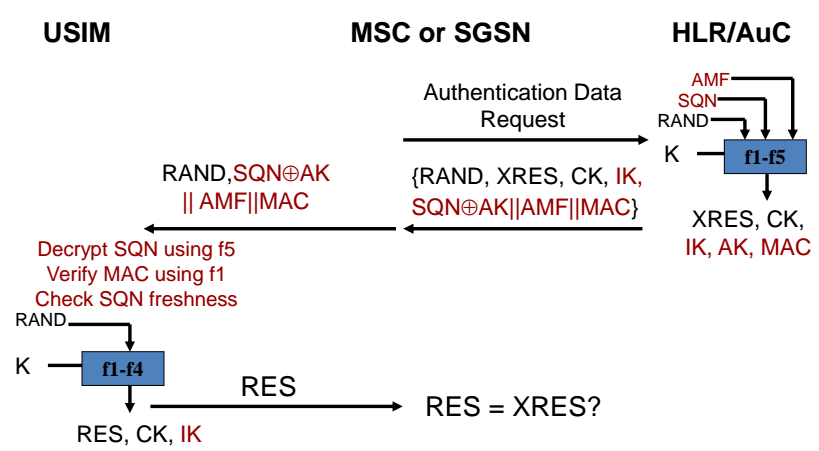
\includegraphics[scale=0.2]{UMTS_Authentication_Protocol.png}
\caption{UMTS Authentication}
\label{fig:prob2c1}
\end{mdframed}
\end{figure}

\begin{figure}
\begin{mdframed}
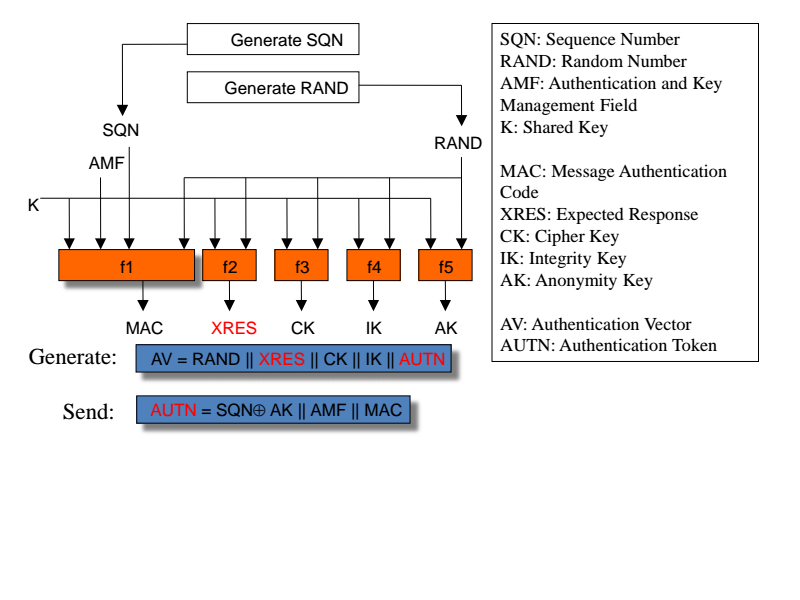
\includegraphics[scale=0.2]{Generation_of_Authentication_Vector.png}
\caption{Generation of Authentication Vector}
\label{fig:prob2c2}
\end{mdframed}
\end{figure}

\begin{figure}
\begin{mdframed}
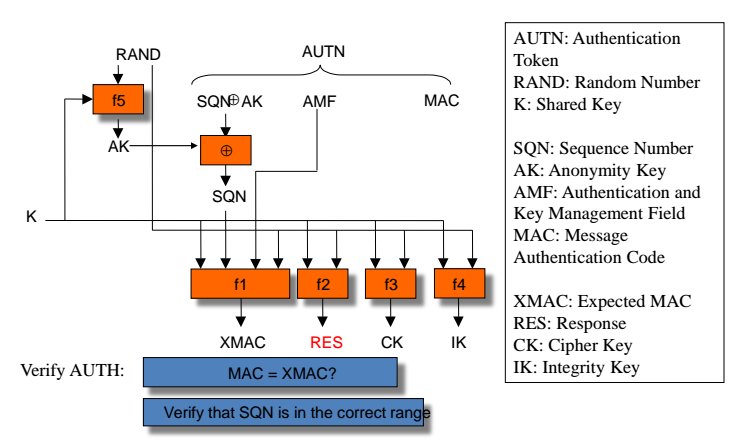
\includegraphics[scale=0.2]{Verification_of_Mobile_Station.png}
\caption{Verification of Mobile Station}
\label{fig:prob2c3}
\end{mdframed}
\end{figure}

%Problem 3
\section{Problem 3 --- Attacks on authentication protocols in GSM Security}

Alice is using GSM cellular network to communicate with her friends.

\subsection{Is it possible for Eve, the attacker, to authenticate herself to the network as the
      legitimate subscriber?}

Yes.

\subsection{Is it possible for the attacker to decrypt all the calls from and to the subscriber?}

Yes.

\subsection{Consider the cases in Problem 3.a and 3.b, how would the attacker successfully
      achieve these goals in \textbf{reality}? (What approaches can the attacker do physically?)}

\end{document}
